\documentclass{article}


% if you need to pass options to natbib, use, e.g.:
%     \PassOptionsToPackage{numbers, compress}{natbib}
% before loading neurips_2023


% ready for submission
\usepackage[final]{neurips_2023}


% to compile a preprint version, e.g., for submission to arXiv, add add the
% [preprint] option:
%     \usepackage[preprint]{neurips_2023}


% to compile a camera-ready version, add the [final] option, e.g.:
%     \usepackage[final]{neurips_2023}


% to avoid loading the natbib package, add option nonatbib:
%    \usepackage[nonatbib]{neurips_2023}

\usepackage[utf8]{inputenc} % allow utf-8 input
\usepackage[T1]{fontenc}    % use 8-bit T1 fonts
\usepackage{hyperref}       % hyperlinks
\usepackage{url}            % simple URL typesetting
\usepackage{booktabs}       % professional-quality tables
\usepackage{amsfonts}       % blackboard math symbols
\usepackage{amsmath}
\usepackage{nicefrac}       % compact symbols for 1/2, etc.
\usepackage{microtype}      % microtypography
\usepackage{xcolor}         % colors
\usepackage{graphicx}
\usepackage{float}
\usepackage{subfig}

\bibliographystyle{plainnat}


\title{ECEN 757 | Homework 3 (Ungraded)}


% The \author macro works with any number of authors. There are two commands
% used to separate the names and addresses of multiple authors: \And and \AND.
%
% Using \And between authors leaves it to LaTeX to determine where to break the
% lines. Using \AND forces a line break at that point. So, if LaTeX puts 3 of 4
% authors names on the first line, and the last on the second line, try using
% \AND instead of \And before the third author name.

\author{%
  Muhammed U. Ersoy\\
  M.S. ECEN Student\\
  Texas A\&M University\\
  \texttt{mue@tamu.edu} \\
 }

\begin{document}
\maketitle

\section{Explain why reversing the order of the lines ‘R-deliver m’ and ‘if (q$\ne$ p ) then B-
multicast(g, m); end if’ in Figure 15.9 makes the algorithm no longer satisfy uniform
agreement. Does the reliable multicast algorithm based on IP multicast satisfy uniform
agreement?}

If the process delivers $m$ to application layer before its' multicast then the process $q$ could potentially 
fail before it delivers the message breaking the uniform agreement.
\begin{figure}[H]
    \centering
    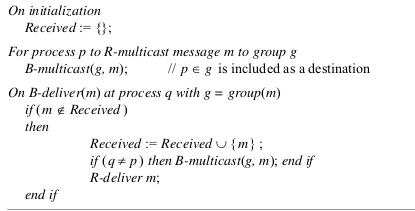
\includegraphics[width=10cm]{fig15_9.png}
    \caption{}
\end{figure}

\section{Show that the FIFO-ordered multicast algorithm does not work for overlapping groups,
by considering two messages sent from the same source to two overlapping groups, and
considering a process in the intersection of those groups. Adapt the protocol to work for
this case. Hint: processes should include with their messages the latest sequence
numbers of messages sent to all groups.}

By default the algorithm does not distinguish between groups in the messages that are multicast. So a process
at the intersection could potentially receive two different messages with the same sequence id. 

To resolve this the messages need to somehow identify which group they are coming from. A simple solution would be to include the entire vector that contains
the greatest sequence number sent for each process from a group.

\section{Show that, if the basic multicast that we use in the algorithm of Figure 15.13 is also
FIFO-ordered, then the resultant totally-ordered multicast is also causally ordered. Is it
the case that any multicast that is both FIFO-ordered and totally ordered is thereby
causally ordered?}

In the sequencer based totally-ordered multicast algorithm a central server keeps track of the global state of multicast messages
via a global montonically increasing counter. This already guarantees the causality relationship between two different processes.
For example, if $p_1$ wants to multicast a message and requests the sequence number from the server, and after multicasting that triggers / causes
an event in $p_2$ that results in a multicast we know that the ordering of messages $m_1 \rightarrow m_2$ is going to satisfy the causality.

The only guarantee that does not exist here is the ordering of messages from the same machine. If we can guarantee that two messages from the same $p_i$
follow the FIFO order then a totally-ordered multicast will satisfy the causality condition for that particular group.

A totally ordered and FIFO multicast algorithm does not always satisfy causality. Totally ordered only cares about all the machines
receiving the messages in the same order but not necessarily in the order it received them. In this case we get causality because the sequencer
algorithm respects the causality of the multicasting process.

\begin{figure}[H]
    \centering
    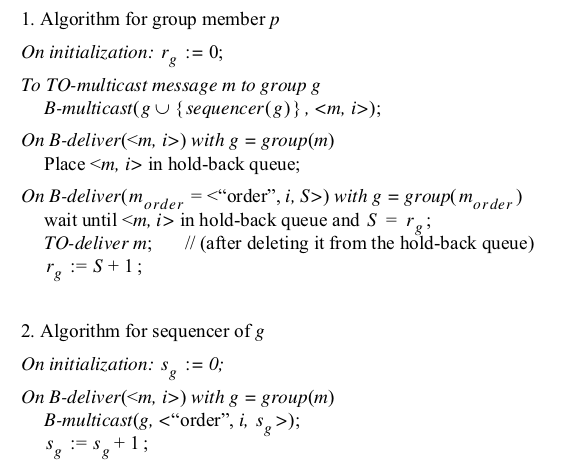
\includegraphics[width=10cm]{fig15_13.png}
    \caption{}
\end{figure}
ordering
\section{Consider the algorithm given in Figure 15.17 for consensus in a synchronous system,
which uses the following integrity definition: if all processes, whether correct or not,
proposed the same value, then any correct process in the decided state would chose that
value. Now consider an application in which correct processes may propose different
results, e.g., by running different algorithms to decide which action to take in a control
system’s operation. Suggest an appropriate modification to the integrity definition and
thus to the algorithm.}

We could use a majority rule meaning whichever process gets the more votes they win the election. If there is
a tie, we can use the unique identifier of that process with a max function as the tie breaker.

\section{Show that Byzantine agreement can be reached for three generals, with one of them
faulty, if the generals digitally sign their messages.}

Cryptographic signatures can be assumed to be unforgable and authentic. When a general sends an authentic message
and the traitor sends / relays a forged message we can verify whether the message that is being relayed
is authentic and from a general.

\bibliography{default}
\end{document}


